\chapter{Reuse}\label{reuse}

Up to this point, the aspect of control dominates the exposition. We 
have essentially been interested in the reactive code. The 
foundations of synchronous programming are settled by now, and we can 
proceed to a more structural, object-oriented view. 

\section{Interfacing Reactive Objects.}\label{signalbus}
\index{object!reactive}\index{reactive object}

\paragraph{Parameterizing reactive classes.} We reiterate that 
reactive objects communicate by sensors and signals only.  
The interface to the environment has been discussed in in Section~\ref{interface}. Now we focus on interfacing reactive objects. 

Sensors and signals are passed to reactive object by calling
its constructor. Note that reactive objects have only one constructor. 
To give an example, we modify 
the class \pp{Counter} of Subsection~\ref{counter} of 
Chapter~\ref{core}: the sensors and signals become parameters of the
constructor
% 
\codeinput{counter-object}
% 
Instances of reactive classes are created using the operator \pp{new} 
as usual.  Counters are, for instance, used in the class 
\pp{PulseWidthModulation} to modulate a signal \pp{wave} to be ``up'' 
and ``down'' for a specified number of instants.
%
\codeinput{pulse-width-modulation1}
% 
The signal \pp{wave} is emitted with value \pp{true} if the value 
\pp{toHighPhase} is present, and emits the signal \pp{wave} with 
value \pp{false} if the value \pp{toHighPhase} is present. The 
counter \pp{highTimer} counts the instants of the high phase, as 
specified by the actual value of the variable \pp{high}, and the 
counter \pp{lowTimer} counts the instants of the low phase, as 
specified by the actual value of the variable \pp{low}.

The signals \pp{clock}, \pp{toHighPhase}, and to \pp{toLowPhase} are
arguments of the two constructors of the counters. One should note 
that the signals are constrained to be read-only sometimes. For 
instance, the signal \pp{toHighPhase} is restricted to be read-only 
as argument of the counter initializing \pp{highTimer} (since the 
parameter \pp{start} of the counter if of type \pp{ConstSignal}). In 
contrast, the counter initializing \pp{lowTimer} emits the signal 
\pp{toHighPhase} but can only read the signal \pp{toLowPhase}. 

\paragraph{Constructor invocations.}\index{constructor!invocation} The semantics of object 
composition is that, when generating an instance of class 
\pp{PulseWidthModulation}, 
\begin{itemize}
\item signal parameters are substituted by arguments, e.g. the 
signal parameter \pp{start} of a counter is substituted by the signal 
argument \pp{toHighTimer} when initialising of the 
variable \pp{highTimer}.

\item the reactive code of the object \pp{PulseWidthModulation} and of
all its reactive subobjects -- here the two counters 
\pp{highTimer} and \pp{lowTimer} -- are put in parallel.
\end{itemize}

The resulting reactive code is (more or less) equivalent to
%
\codeinput{pulse-width-modulation2}
% 
Some renaming has been used: for instance, the method \pp{reset} of the
class \pp{Counter}  has two  ``localised'' versions \pp{resetHigh} and \pp{resetLow} to mimic the objects \pp{highTimer} and \pp{lowTimer}.


\paragraph{Objects and Multiple Emittance}\index{precedences, signals and objects}

Since reactive objects evaluate in parallel, and since they may share signals, conflicts may arise due to multiple emittance. Consider the following (rather useless) object
%
\codeinput{multiple-emittance1}
% 
which is instantiated twice
%
\codeinput{multiple-emittance2}
% 
Hence the signal \pp{result} is emitted twice at the first instant, with the value $3$ and with value $5$. An error message \pp{MultEmitInAppl} is raised. Since the error concerns several objects, precedence rules as defined so far will fail to cope. We introduce a new kind of precedence is introduced:
%
\codeinput{multiple-emittance3}
%
It states that if the signal \pp{result} is emitted in both the objects \pp{simple1} 
and \pp{simple2}, the \emph{every} emittance of the signal in \pp{simple1} precedes
any emmittance of the signal in \pp{simple2}.



\section{The Signal Bus}\index{signal bus}
\paragraph{Pictorial presentation.} If we focus on the reactive part 
of objects, a pictorial presentation may be illuminating. Let an 
instance of the class \pp{Counter} be sketched by
\begin{center}
   \setlength{\unitlength}{0.9pt}   
   \begin{picture}(160,90)
   \put(0,0){\framebox(160,80)}
   \put(10,10)
   {\small
   \begin{picture}(140,65)

      \put(25,70){\vector(0,-1){35}}
      \put(0,60){\scriptsize\texttt{start}}
      \put(60,70){\vector(0,-1){35}}
      \put(35,60){\scriptsize\texttt{clock}}
      \put(110,35){\vector(0,1){35}}
      \put(115,44){\scriptsize\texttt{elapsed}}
       
      \put(10,0)
       {\begin{picture}(120,35)
          \put(35,15){\scriptsize\textit{reactive code}}
          \dashline[28]{5}(0,0)(120,0)
          \dashline[28]{5}(0,0)(0,35)
          \dashline[28]{5}(0,35)(120,35)
          \dashline[28]{5}(120,0)(120,35)
       \end{picture}}
   \end{picture}}
 \end{picture}
\end{center}
Its reactive code is indicated by the dashed box, and the object 
itself by the framed box (forgetting about data fields and methods) 
The parameter signals are presented by arrows going from the framed 
box to the dashed box and vice versa.

The reactive structure of an instance of class 
\pp{PulseWidthModulation} may be then presented by
\begin{center}
\begin{picture}(335,135)
\put(0,0){\framebox(335,130)}

 \put(10,80){\line(1,0){315}} 
 \put(10,90){\line(1,0){315}} 
 \put(10,100){\thicklines\vector(1,0){325}} 
 \put(0,110){\thicklines\line(1,0){325}} 
 \put(1,110){\thicklines\vector(1,0){5}} 
 \put(0,120){\thicklines\line(1,0){325}} 
 \put(1,120){\thicklines\vector(1,0){5}} 
 \put(10,122){\footnotesize clock}
 \put(10,112){\footnotesize start}
 \put(305,102){\footnotesize wave}
 \put(100,92){\scriptsize toHighPhase}
 \put(220,82){\scriptsize toLowPhase}
 
 \put(20,110){\vector(0,-1){60}}
 \put(30,90){\vector(0,-1){40}}
 \put(40,80){\vector(0,-1){30}}
 \put(70,50){\vector(0,1){50}}

 \put(127,90){\vector(0,-1){46}}
 \put(150,120){\vector(0,-1){76}}
 \put(185,44){\vector(0,1){40}}

 \put(247,80){\vector(0,-1){36}}
 \put(270,120){\vector(0,-1){76}}
 \put(305,44){\vector(0,1){46}}

\put(5,5){\tiny PulseWidthModulation}

\put(5,5) {
 \begin{picture}(335,140)
       \put(0,0) {\scriptsize
       \begin{picture}(120,35)
          \put(15,25){\textit{reactive code}}
          \dashline[28]{5}(0,10)(80,10)
          \dashline[28]{5}(0,10)(0,45)
          \dashline[28]{5}(0,45)(80,45)
          \dashline[28]{5}(80,20)(80,45)
       \end{picture}}
            
  \put(80,0){
   \setlength{\unitlength}{0.7pt}
   \tiny
   \begin{picture}(160,110)  
   
   \put(0,0){\framebox(160,90)}
   \put(10,10)
   {\tiny
   \begin{picture}(140,65)
      \put(10,10)
       {\begin{picture}(120,35)
          \put(30,15){\scriptsize\textit{reactive code}}
          \dashline[28]{5}(0,0)(120,0)
          \dashline[28]{5}(0,0)(0,35)
          \dashline[28]{5}(0,35)(120,35)
          \dashline[28]{5}(120,0)(120,35)
       \end{picture}}
    \end{picture}}
    \put(5,5){highTimer}
  \end{picture}}
 \put(200,0){
   \setlength{\unitlength}{0.7pt}
   \tiny
   \begin{picture}(160,110)  
   
   \put(0,0){\framebox(160,90)}
   \put(10,10)
   {\tiny
   \begin{picture}(140,65)
      \put(10,10)
       {\begin{picture}(120,35)
          \put(30,15){\scriptsize\textit{reactive code}}
          \dashline[28]{5}(0,0)(120,0)
          \dashline[28]{5}(0,0)(0,35)
          \dashline[28]{5}(0,35)(120,35)
          \dashline[28]{5}(120,0)(120,35)
       \end{picture}}
    \end{picture}}
    \put(5,5){lowTimer}
  \end{picture}}
 \end{picture}}
\end{picture}
\end{center}
The picture suggests that the reactive codes of the objects involved 
are executed in parallel and that the different fragments of code 
communicate via a bundle of signals. We speak of a \emph{signal bus} 
to refer to this bundle. The signal bus is comprised of all signal 
(fields) specified in a class. We distinguish local signals such as 
\pp{toHighPhase} and \pp{toLowPhase}, input signals such as 
\pp{clock} and \pp{start}, and output signals such as \pp{wave}. We 
distinguish input and outputs to the environment by a thicker line, 
and indicate the interface to the environment by connecting them to 
the vertical sides of the framed box (while parameter signals are 
connected to the top of the box). 

The \se-logo\index{\se-logo}
\begin{center}
    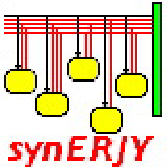
\includegraphics[width=40pt]{../pdf/se-logo}    
\end{center}
is meant to visualize the idea of a \emph{signal bus}.


%We may give an UML object diagram of the same configuration which 
%tells less, though.
%\begin{center}
%   {\tt\scriptsize
%   \setlength{\unitlength}{0.9pt}
%   \begin{picture}(370,190)

%   \put(0,75){\framebox(60,40){\underline{:PulseW\ldots}}}
%   \put(40,115){\vector(1,1){60}} 
%   \put(40,75){\vector(1,-1){60}} 
%   \put(15,120){\tiny highTimer}
%   \put(15,65){\tiny lowTimer}

%   \put(55,115){\vector(2,1){125}} 
%   \put(55,120){\tiny toHighPhase}   
%   \put(60,98){\vector(3,1){120}} 
%   \put(80,110){\tiny start}   
%   \put(60,95){\vector(1,0){120}} 
%   \put(90,97){\tiny clock}   
%   \put(60,92){\vector(3,-1){120}} 
%   \put(80,78){\tiny wave}   
%   \put(55,75){\vector(2,-1){125}} 
%   \put(55,68){\tiny toLowPhase} 
%   
%   \put(100,160){\framebox(40,30){\underline{:Timer}}}
%   \put(100,0){\framebox(40,30){\underline{:Timer}}}   
%   
%   \put(140,15){\vector(1,4){40}} 
%   \put(130,50){\tiny start}   
%   \put(140,175){\vector(1,-4){40}} 
%   \put(130,140){\tiny start}   
%   \put(140,5){\vector(1,0){40}} 
%   \put(142,0){\tiny elapsed}   
%   \put(140,185){\vector(1,0){40}} 
%   \put(142,187){\tiny elapsed}   
%   \put(140,10){\vector(1,2){40}} 
%   \put(144,175){\tiny clock}   
%   \put(140,180){\vector(1,-2){40}} 
%   \put(144,13){\tiny clock}   
%   
%   
%   \put(180,160){\framebox(80,30){\underline{:Signal}}}
%   \put(180,120){\framebox(80,30){\underline{:ConstSignal}}}
%   \put(180,80){\framebox(80,30){\underline{:ConstSignal}}}
%   \put(180,0){\framebox(80,30){\underline{:Signal}}}
%   \put(180,40){\framebox(90,30){\underline{:Signal<boolean>}}}
%   \put(260,135){\vector(1,0){30}} 
%   \put(260,95){\vector(1,0){30}} 
%   \put(270,55){\vector(1,0){20}} 
%   
%   \put(290,120){\framebox(50,30){\underline{:Input}}}
%   \put(290,80){\framebox(50,30){\underline{:Input}}}
%   \put(290,40){\framebox(50,30){\underline{:Output}}}

% \end{picture}}
%\end{center}
%We see that all the signals of an object of type 
%\pp{PulseWidthModulation} 
%are aliased with signals of the respective subobjects. This is how 
%the 
%wiring of signals is presented from the object-oriented perspective. 

  
\paragraph{Signal bus hierarchy.} Reactive objects and signal busses 
naturally form hierarchies.\index{hierarchy}\index{signal bus!hierarchy}
 Consider, for instance, a variant of the 
\pp{Counter} class.
%
\codefragment{counter-parameter-fragment}
%
Here the parameters are used to initialize the signals \pp{start}, 
\pp{clock}, and \pp{elapsed}. The corresponding graphics is
\begin{center}
   \begin{picture}(160,110)
   \put(13,93){\scriptsize\texttt{\_start}}
   \put(40,100){\vector(0,-1){20}}
   \put(58,93){\scriptsize\texttt{\_clock}}
   \put(85,100){\vector(0,-1){30}}
   \put(105,93){\scriptsize\texttt{\_elapsed}}
   \put(140,60){\vector(0,1){40}}
   
   \put(0,0){\framebox(160,100)}
   \put(10,10)
   {\small
   \begin{picture}(140,65)
      \put(0,50){\line(1,0){140}} 
      \put(0,60){\line(1,0){140}} 
      \put(0,70){\line(1,0){140}}

      \put(25,70){\vector(0,-1){35}}
      \put(0,64){\scriptsize\texttt{start}}
      \put(60,60){\vector(0,-1){25}}
      \put(35,54){\scriptsize\texttt{clock}}
      \put(110,35){\vector(0,1){15}}
      \put(115,44){\scriptsize\texttt{elapsed}}
       
      \put(10,0)
       {\begin{picture}(120,35)
          \put(35,15){\scriptsize\texttt{loop \{ \ldots\ \};}}
          \dashline[28]{5}(0,0)(120,0)
          \dashline[28]{5}(0,0)(0,35)
          \dashline[28]{5}(0,35)(120,35)
          \dashline[28]{5}(120,0)(120,35)
       \end{picture}}
   \end{picture}}
 \end{picture}
\end{center}
The signal bus is comprised of the signal fields that are used inside 
the reactive code and that are connected to the parameters. Using 
this kind of counter the composition of objects yields the following 
hierarchy where each object has a local signal bus.\index{signal bus!local}
\begin{center}
\begin{picture}(335,140)
\put(0,0){\framebox(335,130)}

 \put(10,80){\line(1,0){315}} 
 \put(10,90){\line(1,0){315}} 
 \put(10,100){\thicklines\vector(1,0){325}} 
 \put(0,110){\thicklines\line(1,0){325}} 
 \put(1,110){\thicklines\vector(1,0){5}} 
 \put(0,120){\thicklines\line(1,0){325}} 
 \put(1,120){\thicklines\vector(1,0){5}} 
 \put(10,122){\footnotesize clock}
 \put(10,112){\footnotesize start}
 \put(305,102){\footnotesize wave}
 \put(100,92){\scriptsize toHighPhase}
 \put(220,82){\scriptsize toLowPhase}
 
 \put(20,110){\vector(0,-1){60}}
 \put(30,90){\vector(0,-1){40}}
 \put(40,80){\vector(0,-1){30}}
 \put(70,50){\vector(0,1){50}}

 \put(127,90){\vector(0,-1){29}}
 \put(150,120){\vector(0,-1){66}}
 \put(185,47){\vector(0,1){33}}

 \put(247,80){\vector(0,-1){19}}
 \put(270,120){\vector(0,-1){66}}
 \put(305,47){\vector(0,1){33}}

\put(5,5){\tiny PulseWidthModulation}

   
\put(5,5) {
 \begin{picture}(335,140)
       \put(0,0) {\scriptsize
       \begin{picture}(120,35)
          \put(15,25){\textit{reactive code}}
          \dashline[28]{5}(0,10)(80,10)
          \dashline[28]{5}(0,10)(0,45)
          \dashline[28]{5}(0,45)(80,45)
          \dashline[28]{5}(80,10)(80,45)
       \end{picture}}
            
  \put(80,0){
   \setlength{\unitlength}{0.7pt}
   \tiny
   \begin{picture}(160,110)  
   
   \put(0,0){\framebox(160,90)}
   \put(10,10)
   {\tiny
   \begin{picture}(140,65)
      \put(0,50){\line(1,0){140}} 
      \put(0,60){\line(1,0){140}} 
      \put(0,70){\line(1,0){140}} 

      \put(25,70){\vector(0,-1){35}}
      \put(0,64){\texttt{start}}
      \put(60,60){\vector(0,-1){25}}
      \put(35,54){\texttt{clock}}
      \put(110,35){\vector(0,1){15}}
      \put(115,44){\texttt{elapsed}}
       
      \put(10,0)
       {\begin{picture}(120,35)
          \put(20,15){\scriptsize\textit{reactive code}}
          \dashline[28]{5}(0,0)(120,0)
          \dashline[28]{5}(0,0)(0,35)
          \dashline[28]{5}(0,35)(120,35)
          \dashline[28]{5}(120,0)(120,35)
       \end{picture}}
    \end{picture}}
    \put(1,1){highTimer}
  \end{picture}}
 \put(200,0){
   \setlength{\unitlength}{0.7pt}
   \tiny
   \begin{picture}(160,110)  
   
   \put(0,0){\framebox(160,90)}
   \put(10,10)
   {\tiny
   \begin{picture}(140,65)
      \put(0,50){\line(1,0){140}} 
      \put(0,60){\line(1,0){140}} 
      \put(0,70){\line(1,0){140}} 

      \put(25,70){\vector(0,-1){35}}
      \put(0,64){\texttt{start}}
      \put(60,60){\vector(0,-1){25}}
      \put(35,54){\texttt{clock}}
      \put(110,35){\vector(0,1){15}}
      \put(115,44){\texttt{elapsed}}
       
      \put(10,0)
       {\begin{picture}(120,35)
          \put(20,15){\scriptsize\textit{reactive code}}
          \dashline[28]{5}(0,0)(120,0)
          \dashline[28]{5}(0,0)(0,35)
          \dashline[28]{5}(0,35)(120,35)
          \dashline[28]{5}(120,0)(120,35)
       \end{picture}}
    \end{picture}}
    \put(1,1){lowTimer}
  \end{picture}}
 \end{picture}}
\end{picture}
\end{center}
The pictures are meant to suggest that
\begin{itemize}
  \item reactive objects and signal busses form a static hierarchy, 
and that

  \item if signals of different busses are "wired" together, it is 
sufficient to generate only one signal (we refer to as 
\emph{principal signal}\index{signal!principal}) and to replace every signal by its principal 
signal.
\end{itemize} 
We will analyse these requirements more deeply in 
Section~\ref{firewalls}.

\paragraph{Configuration classes.} 
Reactive classes without parameters are considered as potential configuration classes. A configuration class\index{configuration class}\index{class!configuration} generates an executable in that itself and all the reactive classes below in the static hierarchy of reactive classes are ``wired'' are wired to form one application.

A configuration class must be chosen explicitly if there is more than one candidate (using a combobox in the \se\ programming environment). A configuration class must be chosen explicitly if there is more than one candidate (using a combobox In the \se\ programming environment \cite{userguide})).

One should note that candidates for a configuration class may be below each other within the static hierarchy.


\paragraph{On input and output signals.} 
We like to stress that every reactive object may specify input sensors\index{sensor!input} and output signals\index{signal!output}. This is in contrast to the more usual idea that input and output signals are defined only top-level
by the configuration object (i.e. the only object generated by a configuration class).


There are good reasons: imagine an application with some component 
being a key pad for submitting a personal identification number.  The 
design of such pads may vary, even in terms of the number of inputs.  
However, the number of inputs usually is irrelevant with regard to 
the overall application that may only depend on whether a correct pin 
has been submitted. 

A schematic view of the key pad control in terms of the interface may 
be
\begin{center}
  \begin{picture}(180,120)
    \put(0,0){\framebox(180,110){}}
    \put(5,68){\footnotesize accept}
    \put(1,65){\thicklines\vector(1,0){5}}
    \put(0,65){\thicklines\line(1,0){170}}
    \put(5,78){\footnotesize bn}
    \put(1,75){\thicklines\vector(1,0){5}}
    \put(0,75){\thicklines\line(1,0){170}}
    \put(3,85){\ldots}
    \put(5,98){\footnotesize b1}
    \put(1,95){\thicklines\vector(1,0){5}}
    \put(0,95){\thicklines\line(1,0){170}}
    \put(150,58){\footnotesize receipt}
    \put(10,55){\thicklines\vector(1,0){170}}
    \put(63,103){\footnotesize reset}
    \put(85,110){\vector(0,-1){70}}    
    \put(100,103){\footnotesize pin}
    \put(95,40){\vector(0,1){70}}    

    \put(40,95){\vector(0,-1){55}} 
    \put(50,75){\vector(0,-1){35}} 
    \put(60,65){\vector(0,-1){25}} 
    \put(140,40){\vector(0,1){15}}    
    
    \put(30,5)
     {\begin{picture}(120,35)
        \put(35,15){\small\textit{reactive code}}
        \dashline[28]{5}(0,0)(120,0)
        \dashline[28]{5}(0,0)(0,35)
        \dashline[28]{5}(0,35)(120,35)
        \dashline[28]{5}(120,0)(120,35)
     \end{picture}}

  \end{picture}    
\end{center}
Here \pp{pin} is meant to be a integer valued signal. The 
box/reactive 
object analyses the sequence of pressed keys if an \pp{accept} 
is submitted. If the sequence is submitted the pin is communicated to 
the application, and the \pp{receipt} signal is emitted with an OK 
message, 
otherwise only the \pp{receipt} signal is emitted with an reject 
message. The number of keys is irrelevant for the overall 
application. It depends on the actual pad. Typically it will have ten 
keys, for instance, for an electronic bank till but there might be 
other builds. 

If input and output signals can only be specified at top-level one 
may have to touch many components of an application to pass the 
key signals down to the pin analyser and to pass the receipt signal 
back to top-level. In \se, these variations have only a local impact 
in 
that the component and the connectors have to be redesigned. In that 
the rationale of \se\ is component oriented in that reactive objects 
behave the same within an application even if the interface to the 
environment may differ.


\section{Structural Constraints}\label{firewalls}\index{firewall}

\paragraph{Firewalls for separating concerns.} A design goal of \se\ 
has been clearly to separate of different concerns as there are: 
reactive control, data operations, and interaction of objects. We 
speak of \emph{firewalls} if addressing these separations of 
concern.  The firewalls encapsulate some of the design decision of 
\se. There are three such firewalls:
\begin{description}
    \item[] \emph{Data Firewall}
     -- Control dominates data.

    \item[] \emph{Signal Firewall}
    -- Reactive object only share 
signals. 

%    \item[] \emph{State Firewall} -- Only state information is 
%communicated in distributed synchronous systems.
\end{description}
%The latter will be explained only later in Chapter~\ref{dsp}. 

\paragraph{The data firewall.}
\index{firewall!data}\index{data firewall}
The data firewall avoids dynamic changes of the reactive control.  The
data firewall restricts the use relation in that
\begin{itemize}
    \item A reactive class can only be a subclass of a reactive 
class. 
    
    \item data methods cannot invoke reactive methods.
\end{itemize}
The requirement reflects the standard two-level architecture for 
control  applications: control dominates data.

\paragraph{The signal firewall.}
\index{firewall!signal}\index{signal firewall}
The signal firewall constrains time race analysis of data calls to 
reactive objects, both for reasons of transparency and for reasons of 
efficiency of the semantic analysis. The constraints are that
\begin{itemize}
     \item constructor parameters are either primitive types
     and signal types, and that
    
     \item all fields and methods of a reactive class are private.
\end{itemize}
The combination avoids that two reactive objects can share 
data except for signals.

Note that time races may still occur between signal emittances.  Like
causality, time races can only partly be resolved on the level of a 
class but requires an analysis at the level of an application, at some 
cost in terms of computing time for the semantic analysis.

\paragraph{Control is static.}
\index{staic control}\index{control!static}
 The firewalls are effective due to an 
essential fact: the structure of reactive behaviour is statically 
determined at compile time. Only then our analysis of causality and 
of time races is feasible. Control is static because of several 
constraints.
\begin{itemize}
	\item For each reactive class, the call graph of reactive methods
	is cycle-free.

	\item The call graph of reactive objects forms a tree with the
	configuration object at the root (i.e. the one having the method
	\pp{main}).
    
	\item Subtrees of objects are downwards closed with regard to
	signals: an reactive object can access signals of a super object,
	but not vice versa, i.e. \emph{the signal bus must be properly
	constructed}.

    \item Reactive objects do not share data except for signals.
\end{itemize}

\paragraph{Mapping the signal bus.} 
Using constructor parameters for sharing signals is too general to
implement the signal bus faithfully.  For the signal bus, we have to
guarantee that there is exactly one signal that corresponds to one
wire.

For a proper implementation of the signal bus\index{signal bus!implementation}, a signal variable  
must be constrained to refer to a signal of the following kinds:
\begin{itemize}
    \item  a \emph{local} signal, or

    \item  an \emph{input} or \emph{output} signal,

    \item  a \emph{global} signal of a super object.
\end{itemize}
We speak of local and input/output signals as \emph{principal
signals}\index{signal!principal}
 of the respective object. By induction, a global signal is a 
principal signal of some super object. 

This constraint is syntactically enforced by requiring that
\begin{enumerate}
    
	\item a signal can be assigned to only once. 
    
    \item the assignment to a signal only occurs in its declaration or
    in a constructor tail.  A \emph{constructor tail}
    \index{constructor!tail} consists of a
    sequence of (unconditional) signal assignments followed by
     the active statement.

    \item an assignment to a signal variable is either of the forms
    \begin{quote}
        \texttt{\textit{signal\_variable} = new
        \textit{signal\_constructor}(\ldots);}\\
        \texttt{\textit{signal\_variable} = 
\textit{formal\_parameter};}
    \end{quote}

    \item a signal constructor only occurs in an assignment or
    initializer of the form
    \begin{quote}
        \texttt{\ldots\ \textit{signal\_variable} = new
        \textit{signal\_constructor}(\ldots);}
    \end{quote}
    In that case we refer to \textit{signal\_variable} as a
    \emph{principal signal}\index{signal!principal}.
 
\end{enumerate}
Condition 1 states that at most one value can be assigned to a signal
(variable).  Conditions 2 and 3 state that
\begin{itemize}
    \item a signal (variable) is either initialized using class
    instance generation (\pp{new \ldots}) (this is a principal signal)
    \emph{principal signal}, or that

    \item a signal being argument of the constructor is assigned to
    a signal variable.
\end{itemize}
By induction, every signal argument of a constructor is the principal
signal of some super object.  Hence every signal variable refers to
principal signals, which faithfully reflects the signal wiring of the
visual presentation.  Finally, condition 4 guarantees that ``all
signals are principal''; all signal (objects) are refered to by a
signal (variable).

\section{\textit{A Loophole in the Signal 
Firewall}}\label{trespassing}\index{firewall!loophole}\index{loophole}
{\em

\paragraph{\textit{An example}} In spite of the signal firewall, 
there might be a time race of data methods being invoked in different 
objects. Consider a configuration consisting of a ``sender'' and a ``receiver'' 
\codefragment{Sender}
\codefragment{Receiver}
The configuration class just establishes a connection between a 
sender and two receivers.  
\codefragment{Signalbus}
The class \emph{\pp{Data}} has just a field \emph{\pp{value}} that 
can be updated.
\codefragment{Data}

The behaviour is thus: at the first instant, \emph{\pp{sender}}
\begin{enumerate}
	\item[1.] updates the fields of \emph{\pp{data}} to $0$ ,

	\item[2.]  emits the shared signal \emph{\pp{sig}} with value 
	\emph{\pp{data}}, and

    \item[3.]  updates the fields \emph{\pp{val}} of 
\emph{\pp{data}} to
    $3$. 
\end{enumerate}
In parallel,
\begin{enumerate}
	\item[4.] \emph{\pp{receiver1}} updates the fields of 
\emph{\pp{data}}  	to $1$, and
	\item[4.] \emph{\pp{receiver2}} updates the fields of 
\emph{\pp{data}}  	to $2$.
\end{enumerate}
In contrast to what we aim for, there are time races between the 
various invocations of the method \pp{set}.
 
\paragraph{\textit{Dealing with the problem.}} 
Signals with values of class type allow to transmit complex data 
which clearly is a useful feature. The prize to pay is time races
may occur across object borders.

There are several strategies of how to avoid such time races. Remember once
a signal is updated, its value should not change any more, but only be read 
(\emph{write-before-read}). This trivially holds for values primitive 
type. For values of class type, one should only be able to access
its fields but not to change them. The same holds for arrays.

In other languages than \java\ this is achieved using a class modifier \pp{const} that defines a superclass comprising only those methods 
that are read-only. Hence emittance of signal with a value of class type
should emit a copy obtained by the respective ``const''\index{const} type. 
In that case the three applications of the method \pp{set} would 
be illegal. However, it would be legal to apply to replace the line
\BEP
\$sent.set(3):
\EEP
of the class \pp{Sender} by the line
\BEP
data.set(3):
\EEP
without changing semantic content. 

An alternative strategy would be to guarantee by an in-depth data analysis
that a signal value is not changed once the signal has been emitted/constrained.

Neither of these strategies is currently implemented in \se. Hence we must
leave it as an \textbf{obligation for the programmer} to pursue either of the
strategies:
\begin{itemize}
\item Either explicitly to design ``const'' classes without side effects,
 and to restrict signal values to these, 

\item or otherwise to guarantee that signal value is not changed after emittance.
\end{itemize}

}


%\section{Abstract Reactive Classes}
%A class is reactive if
%\begin{itemize}
%    \item  it has a reactive constructor, i.e. the constructor tail 
%            of the form
%           \begin{center}
%				\pp{active \{ \ldots\ \}},
%            \end{center}
%    \item  it comprises a signal declaration (cf. this section), or

%    \item  a reactive methods (cf. Section~\ref{methods}).

%    \item  the modifier \pp{reactive} is used. (cf. Section~\ref{methods}).
%\end{itemize}
%If a reactive class does not have a reactive constructor it is an {\em abstract reactive class}. The idea is that a reactive class may inherit signal declarations and reactive methods without being ``executable''. Since we expect that an instance of a reactive class generates reactive code, and since reactive code is only generated from within the \pp{active} statement it seems reasonable to consider reactive classes without an reactive constructor as abstract; no instances can be generated. 

%Here is a small example

%\ldots

%Abstract reactive classes are particularly useful in the context of data flow. As discussed in Chapter~\ref{data-flow} data flow specifications are modularized using nodes as  building blocks. Typically data flow specifications share such building blocks that are elementary (such as the raising edge node). All these elementary nodes -- and, of course, others which are shared -- may be zusamenfassen in some abstract reactive class from which other reactive classes inherit. E.g.

%\section{Examples}

%%\subsection{A Traffic Light Controller}

%

%\subsection{A Production Cell}

%\paragraph{The setup.} The production cell consists of a robot that 
%assembles parts as in Figure~\ref{fallstudie}. The case study has 
%been proposed in \cite{kowalewski}.
%\begin{center}
%\begin{figure}[h]
%  \includegraphics[width=280pt]{../pdf/atp-production-cell}
%  \caption{The Production Cell}
%  \label{fallstudie}
%\end{figure}% 
%\end{center}

%\paragraph{The components.}
%Figure~\ref{fallstudie} suggests to consider the robot, the conveyor belt,
%and the storage as components that are complemented by a central control. 

%We now have to decide  which components are considered as being part of
%the control system, and which components are considered as being 
%part of the environment (plant), the latter being only needed to close
%the system for simulation. We here take the view that the storages and
%the central control are part of the system while the robot and the belt
%are part of the environment. The decision is temporary and may be revised
%at any time. We first model the components of both, the system and the environment.
% 
%\paragraph{The storage.}
%The storage is modelled by a class \pp{Stock} as below
%%
%\codeinput{atp-stock}
%%
%The reactive behaviour consists of two parallel processes. The upper
%one models book-keeping. This, being a sort of continuous 
%behaviour, is best modelled using the flow equations. 
%Parts can be added or withdrawn. A sensor \pp{newPart} checks for
%the presence of a new part. If it is present we increase the stock.
%On the other hand, the stock is decreased if a part is withdrawn by
%the robot. 

%
%Einem Lager k\"{o}nnen Teile hinzugef\"{u}gt oder entnommen werden. 
%Dies modellieren wir in Kode 3 mit Hilfe von Datenfl\"{u}ssen, da die
%Information kontinuierlich berechnet wird.  Dazu passt die 
%Vorstellung
%eines Datenflusses als Sequenz von Werten.

%In einer Datenflussgleichung wird f\"{u}r alle Takte definiert, dass
%die Flussvariable auf der linken den Wert des Ausdrucks auf der
%rechten Seite hat.  So beschreibt zum Beispiel der Fluss \pp{lager}
%die Zahl der gelagerten Montageteile.  Diese ist im ersten Takt $0$
%und wird in sp\"{a}teren Takten aus der Zahl der Teile im vorigen 
%Takt
%(\pp{pre(lager}) sowie den Zu- und Abg\"{a}ngen im jetzigen Takt
%berechnet.\footnote{Wie in \textsc{Lustre}~\cite{lustre} wird auf 
%der linken
%Seite des Operators \pp{->} das Verhalten im ersten Takt, auf der
%rechten Seite das Verhalten in sp\"{a}teren Takten beschrieben.} Der
%Boolesche Fluss \pp{geliefert} wird wahr, wenn im vorigen Takt eine
%Entnahmeanforderung vorlag und das Lager gef\"{u}llt war.  Der Fluss
%\pp{weg} ist gleich dem konstanten Fluss \pp{1..}, wenn ein Teil
%geliefert wurde, und dem Fluss \pp{0..} sonst.  Integer-Konstanten
%werden durch den Operator \pp{..} zu einem konstanten Integer-Fluss. 
%F\"{u}r eine kompakte Darstellung benutzen wir den aus C
%gel\"{a}ufigen Operator \pp{{\it\normalsize c} ?{\it\normalsize t}
%:{\it\normalsize e}} anstelle eines ``\pp{if{\it\normalsize c}
%then{\it\normalsize t} else{\it\normalsize e}}''.

%Der Fluss \pp{platzVoll} zeigt an, ob ein
%Montageteil auf dem Greifplatz liegt.
% 
%\BEP
%  sustain \{
%      hinzu      := (?neuesTeil..) ? (1..) : (0..);
%      geliefert  := pre(?entnahme.. \& lager > 0..);
%      weg        := (geliefert) ? (1..) : (0..);
%      lager      := 0.. -> pre(lager) + hinzu - weg;
%      platzVoll  := lager > 0.. \& geliefert;
%  \};

%\mbox{\footnotesize {\bf
%Kode 3:} Lagerhaltung}
%\EEP
%  
%Sporadisches und kontinuierliches Verhalten wird in dem Beispiel
%kombiniert; wir gehen von der Vorstellung aus, dass ein neu
%produziertes Teil beim Eintritt in das Lager durch eine Lichtschranke
%erkannt wird.  Dieses spontane Ereignis wird durch das Signal
%\pp{neuesTeil} modelliert und durch \pp{?neuesTeil..} f\"{u}r
%die weitere Verarbeitung zu einem Fluss konvertiert.  Dagegen
%l\"{a}sst sich der Zustand \pp{platzVoll} des Greifplatzes eleganter
%durch einen Booleschen Fluss beschreiben, obwohl das Verhalten auf 
%den
%ersten Blick \"{a}hnlich erscheint.

%Die Modellierung ist noch unrealistisch; der Greifplatz bleibt nur
%einen Takt leer.  Wenn wir davon ausgehen, dass kein Sensor f\"{u}r
%den Greifplatz verf\"{u}gbar ist, ist die Annahme sinnvoller, dass 
%der
%Greifplatz erst nach Ablauf einer gewissen Zeitspanne wieder besetzt
%sein kann.  Diese Abstraktion l\"{a}\ss t sich elegant imperativ als
%reaktives Verhalten parallel zum Datenfluss formulieren (Kode 4).
% 
%\BEP
%  [[ sustain \{
%       \ldots
%       platzVoll  := lager > 0.. \& \$zeitVorbei..;
%     \};
%  || loop \{
%       await (\$lager > 0);
%       await fuellZeit;
%       emit zeitVorbei(true);
%       await (\$geliefert);
%       emit zeitVorbei(false);
%     \};
%  ]];

%\mbox{\footnotesize {\bf
%Kode 4:} Lagerhaltung}
%\EEP

%

%

%\paragraph{The signal bus.}
%Figure~\ref{signalbus} specifies the layout of the signal bus of the control system. 
%\begin{center}
%\begin{figure}[h]
% {\tt
%     \setlength{\unitlength}{1.4pt}   
% \begin{picture}(240,100)
%    \put(5,90){\bf Control}
%    \put(30,70){\thicklines \vector(0,-1){30}} 
%    \put(30,40){\thicklines \vector(0,1){30}} 
%    \put(5,10){\framebox(50,30){\it active}}
%    \put(75,100){\vector(0,-1){30}} 
%    \put(78,75){\small\texttt{part}}
%    \put(145,100){\vector(0,-1){30}} 
%    \put(110,75){\small\texttt{beltSpeed}}
%    \put(175,70){\vector(0,1){30}} 
%    \put(178,93){\small\texttt{problem}}
%    \put(10,70){\thicklines \line(1,0){240}} 
%    \put(0,0){\thicklines\framebox(260,100)}
%    \put(100,70){\vector(0,-1){30}} 
%    \put(46,45){\small cPartWithdrawn}    
%%    \put(100,23){\footnotesize withdrawal}    
%    \put(105,40){\vector(0,1){30}} 
%%    \put(110,35){\vector(0,1){5}} 
%    \put(107,62){\small cPartAvailable} 
%%    \put(110,35){\footnotesize partAvailable}    
%    \put(70,25){\vector(1,0){25}}     
%    \put(60,17){\small c.newPart}
%    \put(95,10){\thicklines\framebox(50,30){}}
%    \put(97,22){\small\bf Stock cParts}
%    \put(197,70){\vector(0,-1){30}} 
%    \put(143,45){\small dPartWithdrawn}    
%%    \put(200,28){\footnotesize withdrawal}    
%    \put(202,40){\vector(0,1){30}} 
%    \put(203,62){\small dPartAvailable}    
%    \put(170,25){\vector(1,0){25}}     
%%    \put(205,35){\footnotesize partAvailable}    
%    \put(160,17){\small d.newPart}
%    \put(195,10){\thicklines\framebox(50,30){}}
%    \put(197,22){\small\bf Stock dParts}
% \end{picture}}
%  \caption{The Signal Bus}
%  \label{signalbus}
%\end{figure}
%\end{center}
%The reactive object \pp{control} has two sub-objects \pp{cParts} and \pp{dParts} of type \pp{Stock} that model the respective stocks. 

%A stock
%has parameter \pp{withdrawn}, being a sensor, and a parameter \pp{partAvailable} being a signal. 

%The signals \pp{cPartWithdrawn} and \pp{cPartAvailable} replace the parameters  
%Dieser besteht aus einem B\"{u}ndel von
%Signal(leitung)en, das durch die dickere Linie angedeutet wird.  Die
%Signale des Busses k\"{o}nnen in dem aktiven Teil der Steuerung
%gelesen oder geschrieben werden.  Zum B\"{u}ndel geh\"{o}rige Signale
%wie \pp{cEntnahme} und \pp{cGreifPlatzVoll} werden dem Konstruktor 
%der
%Klasse \pp{Lager} mitgegeben, um ein Lager in seine Umgebung
%einzupassen.  Die Modularisierung in \se\ l\"{a}sst also sowohl
%abgeschlossene Komponenten als auch deren hierarchische Verfeinerung
%zu.

%Man beachte, dass jedes reaktive Objekt mit Hilfe lokaler Signale
%\"{u}ber Eingabe- und Ausgabeobjekte mit der Umgebung kommunizieren
%kann.  So k\"{o}nnen die Lager \pp{c} und \pp{d} unmittelbar 
%\"{u}ber die lokalen Signale \pp{c.neuesTeil}  und \pp{d.neuesTeil} 
%angesprochen werden. Diese Lokalit\"{a}t der Ein- und Ausgabe 
%erh\"{o}ht 
%die Flexibilit\"{a}t des Entwurfs.

%

%
%Wir m\"{u}ssen diese (didaktisch hilfreiche) Fehlentscheidung
%zur\"{u}cknehmen und werden anstelle des Attributs ein Signal
%\pp{problem} verwenden.  Wir ersetzen in dem Kode der Steuerung (Kode
%1) den Aufruf der Methode \pp{setProblem(x)} durch ein \pp{emit 
%signal(x)} und fragen in der Bandeinheit ab, ob ein Problem vorliegt

%\BEP
%loop {
%   emit problem(NO\_PROBLEM);
%   emit bandTempo(100); // motor full speed :-)
%   await \$problem != NO\_PROBLEM;
%   next;
%   emit bandTempo(0);   // turn motor off
%   next;
%   await ?restart;      // problem solved
%};

%\mbox{\footnotesize {\bf
%Kode 6:} Revision von Kode 1}\EEP

%Damit haben wir eine saubere Trennung der avisierten Komponenten 
%erzielt. 

%
%\paragraph{Modelled by a state machine: the assembling line.}
%The robot and the conveyor belt interact for assembling the parts. 
%According to which part arrives either a part of type $C$ or $D$ has 
%to be taken. We specify control in terms of a simple state machine 
%having the states  
%\begin{description}

%\item[``\pp{wait}'':] If a part of type \pp{A} or \pp{B} is arriving then 
%move either to state \pp{assemble\_C} or \pp{assemble\_D}.  Otherwise 
%issue an error message.

%\item[``\pp{assemble\_C}'':] If  there is a part at grab point C,
%  a message is issued that a part has been taken (\pp{cPartTaken}) and that 
%  it is to be assembled (\pp{assembled(\$part)}), and the automaton
%  moves to state \pp{wait}. Otherwise it is checked
%  whether the conveyor belt stand still. If not, an error message is issued  
%  \pp{problem(Status.NO\_PART\_C)}. In any case, the state \pp{assemble\_C}
%  is reentered. The error message is meant to stop the movement of the belt.
%  The assumption that the belt does not need to be stopped for assembling
%  if the appropriate part is available.
%  
%    \item[``\pp{assemble\_D}'':]  analogously
%\end{description}

%The corresponding automaton is specified below. Note that identifiers in
%capital letters such as \pp{PART\_A} oder \pp{MISSING\_C} denote constants. 
%%
%\codefragment{atp-control}
%% 

%We use strong abstractions here. For instance, we indicate the behaviour 
%of the robot by emission of the signal \pp{assembled} only. This is 
%sufficient for a first design, and may be refined later. one might think of 
%reformulating the state \pp{assemble\_C} to
%\BEP
%    state assemble\_C
%       entry \{ emit startRobot(\$part); \}
%       when (?assembled) \{           
%          next state wait; 
%       \} else \ldots
%\EEP
%The signal \pp{startRobot} is emitted when entering state
%\pp{assemble\_C} in which control remains until 
%the robot indicates success by emitting the signal \pp{assembled}.

%The assembly line is encapsulated as an object

%\paragraph{Modelled by an imperative program: the belt control.}

%The conveyor belt is controlled by
%%
%\codefragment{atp-belt-control}
%%
%By emmitting the signal \pp{beltSpeed} the intended speed of
%the belt is set. We assume that an internal controller of the
%belt controls the belt so that it approaches the required 
%speed. Again we use an abstraction. Such a controller may later be designed (for instance, as a PID controller using data flow).
%Hence if the signal \pp{beltSpeed(100)} the motor is accelerated (to full speed). If some problem occurs the belt is slowed down to stop. Then the program waits till the problem is resolved as indicated by the presence of the signal  \pp{restart}.  

%Ob ein Problem vorliegt, wird durch den Aufruf der Booleschen
%(Daten-) Methode \pp{hasProblem} entschieden.  Als Seiteneffekt wird
%dabei das Attribut \pp{problem} auf den Wert \pp{NO\_PROBLEM}
%zur\"{u}ckgesetzt.
% 
%\BEP
%  boolean hasProblem() \{
%     local int p = problem;
%     problem = NO\_PROBLEM;
%     return (p != NO\_PROBLEM);
%  \};
%\EEP
% 

%Schaltet man die beiden Programmst\"{u}cke zur Montage und
%Bandverwaltung parallel, weist der \se\ Kompilierer auf einen 
%Konflikt
%zwischen Aufrufen der Methoden \pp{setProblem} und \pp{hasProblem}
%hin.  Beide k\"{o}nnen in einem Takt gleichzeitig gerufen werden, 
%ohne
%dass die Programmstruktur eine Ablaufordnung festlegt.  Dies 
%f\"{u}hrt
%zu Nichtdeterminismus in der Auswertung.  In einem solchen Falle kann
%der Entwickler die Reihenfolge durch einen Sequenzbefehl festlegen.
% 
%\BEP
%  sequence \{
%     setProblem(int) < hasProblem();
%  \};
%\EEP
% 
%Damit wird in jedem Takt jeder Aufruf der Methode \pp{setProblem} 
%stets
%vor jedem Aufruf der Methode \pp{hasProblem} ausgef\"{u}hrt.  
%Generell
%werden nur Programme akzeptiert, bei denen alle derartige Konflikte
%aufgel\"{o}st sind.  Der erzeugte Kode ist
%deterministisch.\footnote{Der Kompilierer w\"{u}rde ein \"{a}hnliches
%Problem entdecken, wenn einer der \pp{next} Befehle vergessen worden
%w\"{a}re.  Dann k\"{o}nnte das Signal \pp{bandTempo}
%nicht-deterministisch mit dem Wert 0 oder mit dem Wert 100 emittiert
%werden.}

%\paragraph{Modelled by data flow: the storage}

%Einem Lager k\"{o}nnen Teile hinzugef\"{u}gt oder entnommen werden. 
%Dies modellieren wir in Kode 3 mit Hilfe von Datenfl\"{u}ssen, da die
%Information kontinuierlich berechnet wird.  Dazu passt die 
%Vorstellung
%eines Datenflusses als Sequenz von Werten.

%In einer Datenflussgleichung wird f\"{u}r alle Takte definiert, dass
%die Flussvariable auf der linken den Wert des Ausdrucks auf der
%rechten Seite hat.  So beschreibt zum Beispiel der Fluss \pp{lager}
%die Zahl der gelagerten Montageteile.  Diese ist im ersten Takt $0$
%und wird in sp\"{a}teren Takten aus der Zahl der Teile im vorigen 
%Takt
%(\pp{pre(lager}) sowie den Zu- und Abg\"{a}ngen im jetzigen Takt
%berechnet.\footnote{Wie in \textsc{Lustre}~\cite{lustre} wird auf 
%der linken
%Seite des Operators \pp{->} das Verhalten im ersten Takt, auf der
%rechten Seite das Verhalten in sp\"{a}teren Takten beschrieben.} Der
%Boolesche Fluss \pp{geliefert} wird wahr, wenn im vorigen Takt eine
%Entnahmeanforderung vorlag und das Lager gef\"{u}llt war.  Der Fluss
%\pp{weg} ist gleich dem konstanten Fluss \pp{1..}, wenn ein Teil
%geliefert wurde, und dem Fluss \pp{0..} sonst.  Integer-Konstanten
%werden durch den Operator \pp{..} zu einem konstanten Integer-Fluss. 
%F\"{u}r eine kompakte Darstellung benutzen wir den aus C
%gel\"{a}ufigen Operator \pp{{\it\normalsize c} ?{\it\normalsize t}
%:{\it\normalsize e}} anstelle eines ``\pp{if{\it\normalsize c}
%then{\it\normalsize t} else{\it\normalsize e}}''.

%Der Fluss \pp{platzVoll} zeigt an, ob ein
%Montageteil auf dem Greifplatz liegt.
% 
%\BEP
%  sustain \{
%      hinzu      := (?neuesTeil..) ? (1..) : (0..);
%      geliefert  := pre(?entnahme.. \& lager > 0..);
%      weg        := (geliefert) ? (1..) : (0..);
%      lager      := 0.. -> pre(lager) + hinzu - weg;
%      platzVoll  := lager > 0.. \& geliefert;
%  \};

%\mbox{\footnotesize {\bf
%Kode 3:} Lagerhaltung}
%\EEP
%  
%Sporadisches und kontinuierliches Verhalten wird in dem Beispiel
%kombiniert; wir gehen von der Vorstellung aus, dass ein neu
%produziertes Teil beim Eintritt in das Lager durch eine Lichtschranke
%erkannt wird.  Dieses spontane Ereignis wird durch das Signal
%\pp{neuesTeil} modelliert und durch \pp{?neuesTeil..} f\"{u}r
%die weitere Verarbeitung zu einem Fluss konvertiert.  Dagegen
%l\"{a}sst sich der Zustand \pp{platzVoll} des Greifplatzes eleganter
%durch einen Booleschen Fluss beschreiben, obwohl das Verhalten auf 
%den
%ersten Blick \"{a}hnlich erscheint.

%Die Modellierung ist noch unrealistisch; der Greifplatz bleibt nur
%einen Takt leer.  Wenn wir davon ausgehen, dass kein Sensor f\"{u}r
%den Greifplatz verf\"{u}gbar ist, ist die Annahme sinnvoller, dass 
%der
%Greifplatz erst nach Ablauf einer gewissen Zeitspanne wieder besetzt
%sein kann.  Diese Abstraktion l\"{a}\ss t sich elegant imperativ als
%reaktives Verhalten parallel zum Datenfluss formulieren (Kode 4).
% 
%\BEP
%  [[ sustain \{
%       \ldots
%       platzVoll  := lager > 0.. \& \$zeitVorbei..;
%     \};
%  || loop \{
%       await (\$lager > 0);
%       await fuellZeit;
%       emit zeitVorbei(true);
%       await (\$geliefert);
%       emit zeitVorbei(false);
%     \};
%  ]];

%\mbox{\footnotesize {\bf
%Kode 4:} Lagerhaltung}
%\EEP

%
%\paragraph{The overall architecture.} 

%\paragraph{Reaktive Objekte}

%Verhaltenskomponenten werden durch \emph{reaktive Klassen} 
%modelliert. 
%Eine wesentliche Einschr�nkung der so definierten reaktiven Objekte 
%ist,
%dass diese nur \"{u}ber Signale kommunizieren d\"{u}rfen.  Dies
%garantiert, dass keine Interaktion der Objekte \"{u}ber Daten 
%erfolgt.

%Ein (rudiment\"{a}res) Beispiel sei

%\BEP
%class Lager \{ 
%  time fuellZeit;
%  ConstSignal   entnahme;
%  Flow<boolean> platzVoll;
%  ConstSignal   neuesTeil  = new ConstSignal(new Input());
%  \ldots

%  public Lager (    ConstSignal \_entnahme, 
%                 Flow<boolean> \_platzVoll, 
%                          time \_fuellZeit  ) \{
%      fuellZeit = \_fuellZeit;
%      entnahme  = \_entnahme;
%      platzVoll = \_platzVoll;

%      active \{
%         \textit{Verhalten - siehe Kode 4}
%     \};
%  \};
%\}

%\mbox{\footnotesize {\bf
%Kode 5:} Klasse Lager}
%\EEP
% 
%Der Verhaltenskode wird durch die Anweisung \pp{active} in den
%Konstruktor eingebettet.  Signalvariablen werden entweder durch
%Konstruktorparameter (\pp{entnahme}) oder durch ein Signalobjekt
%(\pp{neuesTeil}) initialisiert.  An der Signalvariablen 
%\pp{neuesTeil}
%lassen weitere Besonderheiten festmachen: durch den Typ
%\pp{ConstSignal} wird festgelegt, dass das Signal nur getestet und
%nicht emittiert werden kann.  Durch den Parameter \pp{new Input()}
%wird festgelegt, dass dieses Signal mit der Umgebung kommuniziert (in
%diesem Fall als Input).

%\paragraph{Komponentenbildung}

%Reaktive Objekte verhalten sich wie Komponenten: alle Attribute und
%Methoden sind per Definition privat.  Reaktive Klassen sind nach 
%unten
%abgeschlossen.  Interaktion findet nur \"{u}ber Signale statt und
%niemals \"{u}ber Referenzen.  Damit verhalten sich reaktive
%Objekte in jeder Umgebung gleich.

%Gem�� Bild~\ref{fallstudie} bietet es sich an, die Lager und die
%Bandeinheit als Komponenten zu betrachten, die um eine zentrale
%Steuerungskomponente erg\"{a}nzt werden. Jede Komponente soll wie 
%oben 
%das Lager durch eine reaktive Klasse modelliert werden.

%Als n\"{a}chstes ist zu kl\"{a}ren, welche Komponenten wir als Teil
%des Systems und welche Komponenten wir als Teil der Umgebung
%betrachten, deren Modellierung nur dazu dient, das System f\"{u}r 
%eine
%Simulation abzuschlie\ss en.  Wir treffen hier die Entscheidung, dass
%die Lager und die Steuerung Teil des Systems, die Bandeinheit dagegen
%Teil der Umgebung ist.  Diese Entscheidung ist momentan und l\"{a}sst
%sich jederzeit revidieren, wenn wir zum Beispiel eine ausgefeiltere
%Steuerung der Bandeinheit mit dem Diskriminator und Ortsschalter
%entwickeln.

%Wir m\"{u}ssen aber nun feststellen, dass unsere bisherige
%Modellierung dieser Aufteilung nicht standh\"{a}lt; die
%Steuerung und die Bandeinheit greifen \"{u}ber die Datenmethoden auf 
%dasselbe Attribut \pp{problem} zu. Da reaktive Klassen nach unten 
%abgeschlossen sind, ist dies nur m\"{o}glich, wenn das Verhalten der 
%Steuerung und der Bandeinheit in der gleichen Klasse formuliert 
%sind. 

%Wir m\"{u}ssen diese (didaktisch hilfreiche) Fehlentscheidung
%zur\"{u}cknehmen und werden anstelle des Attributs ein Signal
%\pp{problem} verwenden.  Wir ersetzen in dem Kode der Steuerung (Kode
%1) den Aufruf der Methode \pp{setProblem(x)} durch ein \pp{emit 
%signal(x)} und fragen in der Bandeinheit ab, ob ein Problem vorliegt

%\BEP
%loop {
%   emit problem(NO\_PROBLEM);
%   emit bandTempo(100); // motor full speed :-)
%   await \$problem != NO\_PROBLEM;
%   next;
%   emit bandTempo(0);   // turn motor off
%   next;
%   await ?restart;      // problem solved
%};

%\mbox{\footnotesize {\bf
%Kode 6:} Revision von Kode 1}\EEP

%Damit haben wir eine saubere Trennung der avisierten Komponenten 
%erzielt. 

%\paragraph{Signalbus}

%Komponenten werden \"{u}ber einen sogenannten \emph{Signalbus}
%verbunden.  Die Idee ist, dass sich Signale wie Leitungen verschalten
%lassen.  So wird etwa der Boolesche Fluss \pp{cGreifPlatzVoll} der
%Montagesteuerung mit dem Fluss \pp{platzVoll} des Lagers f\"{u}r
%C-teile verbunden ebenso wie das Signal \pp{cEntnahme} mit dem Signal
%\pp{entnahme}.  Bild 2 mag dies veranschaulichen.
%\begin{figure}[h]
% {\tt
%     \setlength{\unitlength}{0.9pt}   
% \begin{picture}(240,100)
%    \put(5,90){\bf Steuerung}
%    \put(30,70){\thicklines \vector(0,-1){30}} 
%    \put(30,40){\thicklines \vector(0,1){30}} 
%    \put(5,10){\framebox(50,30){\it active}}
%    \put(75,100){\vector(0,-1){30}} 
%    \put(78,84){\scriptsize\texttt{basisTeil}}
%    \put(145,100){\vector(0,-1){30}} 
%    \put(103,93){\scriptsize\texttt{bandTempo}}
%    \put(175,70){\vector(0,1){30}} 
%    \put(178,93){\scriptsize\texttt{problem}}
%    \put(10,70){\thicklines \line(1,0){220}} 
%    \put(0,0){\thicklines\framebox(240,100)}
%    \put(105,70){\vector(0,-1){38}} 
%    \put(65,45){\scriptsize cEntnahme}    
%    \put(107,28){\tiny entnahme}    
%    \put(110,35){\vector(0,1){35}} 
%    \put(112,62){\scriptsize cGreif-}    
%    \put(112,55){\scriptsize PlatzVoll} 
%    \put(112,35){\tiny platzVoll}    
%    \put(70,25){\vector(1,0){25}}     
%    \put(65,17){\scriptsize c.neues}
%    \put(74,9){\scriptsize Teil}
%    \put(95,10){\thicklines\framebox(50,30){}}
%    \put(100,15){\bf Lager c}
%    \put(192,70){\vector(0,-1){38}} 
%    \put(153,45){\scriptsize dEntnahme}    
%    \put(195,28){\tiny entnahme}    
%    \put(197,35){\vector(0,1){35}} 
%    \put(200,62){\scriptsize dGreif-}    
%    \put(200,55){\scriptsize PlatzVoll}    
%    \put(160,25){\vector(1,0){25}}     
%    \put(200,35){\tiny platzVoll}    
%    \put(155,17){\scriptsize d.neues}
%    \put(164,9){\scriptsize Teil}
%    \put(185,10){\thicklines\framebox(50,30){}}
%    \put(190,15){\bf Lager d}
% \end{picture}}
% \caption{Die Klasse Steuerung}
% \label{fallstudie}
%\end{figure}
%Die reaktive Klasse \pp{Steuerung} hat zwei reaktive Unterobjekte
%\pp{c} und \pp{d} vom Typ \pp{Lager}.  Diese lesen von und schreiben
%auf den (lokalen) Signalbus.  Dieser besteht aus einem B\"{u}ndel von
%Signal(leitung)en, das durch die dickere Linie angedeutet wird.  Die
%Signale des Busses k\"{o}nnen in dem aktiven Teil der Steuerung
%gelesen oder geschrieben werden.  Zum B\"{u}ndel geh\"{o}rige Signale
%wie \pp{cEntnahme} und \pp{cGreifPlatzVoll} werden dem Konstruktor 
%der
%Klasse \pp{Lager} mitgegeben, um ein Lager in seine Umgebung
%einzupassen.  Die Modularisierung in \se\ l\"{a}sst also sowohl
%abgeschlossene Komponenten als auch deren hierarchische Verfeinerung
%zu.

%Man beachte, dass jedes reaktive Objekt mit Hilfe lokaler Signale
%\"{u}ber Eingabe- und Ausgabeobjekte mit der Umgebung kommunizieren
%kann.  So k\"{o}nnen die Lager \pp{c} und \pp{d} unmittelbar 
%\"{u}ber die lokalen Signale \pp{c.neuesTeil}  und \pp{d.neuesTeil} 
%angesprochen werden. Diese Lokalit\"{a}t der Ein- und Ausgabe 
%erh\"{o}ht 
%die Flexibilit\"{a}t des Entwurfs.

%\subsubsection{Schlussfolgerungen}

%Wir haben einen ersten Entwurf\footnote{Eine vollst\"{a}ndige
%Dokumentation der Fallstudie findet man unter \cite{at}} der
%Fallstudie vorgestellt und angedeutet, wie Entwurfsentscheidungen
%lokal modifiziert und verfeinert werden k\"{o}nnen.  Das grobe Modell
%ist nicht nur eine (eventuell grafische) Darstellung des Systems.  
%Sie
%ist auch ausf\"{u}hrbar und testbar.  Simulation und Regressionstests
%auf einem Arbeitsplatzrechner zeigen trotz Parallelit\"{a}t wegen des
%Determinismus synchroner Programme das gleiche Verhalten wie auf dem
%Zielrechner.

%Ob ein Nachrichtentechniker Datenfluss bevorzugt oder ob ein 
%Informatiker hierarchische Automaten benutzt, ist eine 
%Entwicklungsentscheidung, die durch die Integration der synchronen 
%Stile verborgen werden kann.

